% Chapter 2

\chapter{Preprocessing} % Main chapter title

\label{Chapter2} % For referencing the chapter elsewhere, use \ref{Chapter1} 

%----------------------------------------------------------------------------------------

% Define some commands to keep the formatting separated from the content 
\newcommand{\keyword}[1]{\textbf{#1}}
\newcommand{\tabhead}[1]{\textbf{#1}}
\newcommand{\code}[1]{\texttt{#1}}
\newcommand{\file}[1]{\texttt{\bfseries#1}}
\newcommand{\option}[1]{\texttt{\itshape#1}}

%----------------------------------------------------------------------------------------

\section{Audio Format}
It was deemed most appropriate to use the compressed MP3 extracted from the MPEG-4 video file for a number of reasons. Although using the uncompressed wav form would present a more faithful reproduction of the audio, and possibly provide more data to train on, the additional complexity far outweighed any possible gains. The MFCC extraction is very sensitive to the [something] and testing on the wav file proved prohibitively long. The space requirements were far larger and approached the file size of the compressed video and audio combined. Furthermore, since the aim is to identify human speech, the lossy mpeg compression regime is explicitly designed to mimic the constraints on human hearing using psychoacoustic modelling, whereby imperceptible frequency ranges, signals with subthreshold amplitudes and frequencies masked by other more dominant frequencies are excluded (Perceptual Coding of Digital Audio), among many other filtering techniques. This process is well-suited to feature extraction for ASR as human speech is naturally adapted to be comprehended by human ears, and vice versa. 

The  spoken  voice  frequency  lies between  300  to  3400  Hertz\cite{Sandanalakshmi} and so telephones sample at 8kHz in order to satisfy the nyquist criterion which defines the sample rate necessary to avoid aliasing, where the sample rate frequency is insufficient to capture the full details of the waveform, to be: $f_{s} > 2B$ (sampling frequency greater than twice the bandwidth). 
The sample rate was chosen to be 16kHz in order to avoid this phenomenon, and since the files are compressed the memory requirements are not excessive.

%----------------------------------------------------------------------------------------

\section{Mel Frequency Cepstral Coefficients}

In order to extract the features most relevant to speech, MFCC’s were chosen due to their robustness to noise compared to another popular feature extraction technique, Linear Predictive Cepstral Coefficient \cite{lpccvsmfcc}. Others have found that it performs less well without some preprocessing but is relatively fast to compute \cite{Shrawankar2013}. MFCC’s are considered the baseline, reliable method and there is a python library (python\_speech\_features) available for computing these, and so this was the method chosen.
This technique also applies pschoacoustic modelling to the signal by applying a series of transformations. 

\begin{figure}[h]
	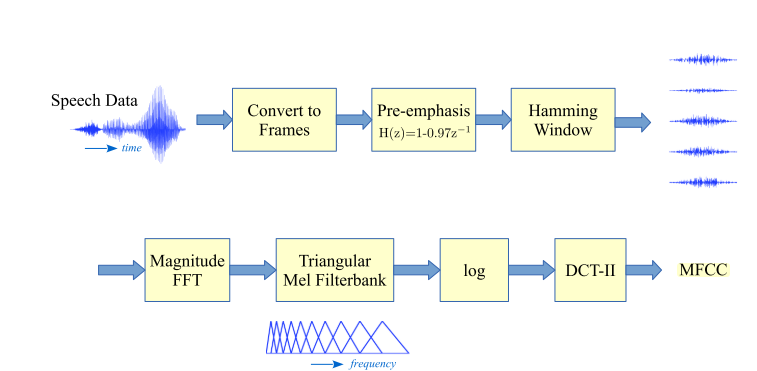
\includegraphics[width=\textwidth]{MFCC_Process}
	\caption{Steps of MFCC Feature Extraction \cite{mfcc_steps}}
	\label{mfcc}
\end{figure}

\subsection{Frame signal into short frames}
The signal is framed into overlapping frames in order for the frequency analysis to be performed. This is assumes that audio spectra are effectively constant over short time frames (typically 20-30ms, ). The windows are overlapping so that continual frequency features are captured...

\subsection{Pre-emphasis}
There is a preemphasis applied, where for each value in the frequency domain a high-pass filter is applied:
\begin{equation}
s_{2}(n) = s(n) - a*s(n-1) 
\end{equation}
where n is the sample number, s is the signal in the frequency domain and s2 is the transformed signal. 
This has 3 effects http://haythamfayek.com/2016/04/21/speech-processing-for-machine-learning.html:
(1) balance the frequency spectrum since high frequencies usually have smaller magnitudes compared to lower frequencies,
(2) avoid numerical problems during the Fourier transform operation and
(3) may also improve the Signal-to-Noise Ratio (SNR).

\subsection{Periodogram}
For each frame the periodogram is calculated, which encapsulates the relative energy in different frequency bands of the signal. This is done using the Discrete Fourier Transform (discrete due to the digital nature of the signal):
\begin{equation}
S_{i}(k) = \sum_{n=1}^{N}  s_{i}(n)h(n)e^{-j2\pi kn/N} \text{for } 1 \leq k \leq K
\end{equation}
where $h(n)$ is an $n$ sample long analysis window (e.g. hamming window), and $K$ is the length of the FFT. For a 16kHz signal in 25ms frames, N equates to 400 samples.
The periodogram-based power spectral estimate for the speech frame  is then given by:
\begin{equation}
P_{i}(k) = \frac{1}{N}|S_{k}|{2}
\end{equation}
i.e. we take the absolute value of the complex fourier transform of each coeffecient, and square the result.

\subsection{Mel Filterbank}
This step applies a series of filters (26 commonly) to the periodogram, composed of vectors of length 26 with nonzero values at different sections along the vector.  The filters are nonuniform, increasing in width with frequency. This emulates the nature of human hearing to have lower sensitivity to changes in frequency as frequency increases. This is based on the Mel scale which models this nonlinearity and describes exactly how to space the bins.
The spectrum $P(f)$ is warped along its frequency axis $f$ (in hertz) into the mel-frequency axis as $P(M)$, where $M$ is the mel-frequency, using:
\begin{equation}
M(f) = 2595 \log((1 + f/700)
\end{equation}
A non-linear frequency scale transformation is applied based on the observation that human hearing does not perceive frequencies linearly but, like amplitude, on a logarithmic scale:
\begin{figure}[h]
	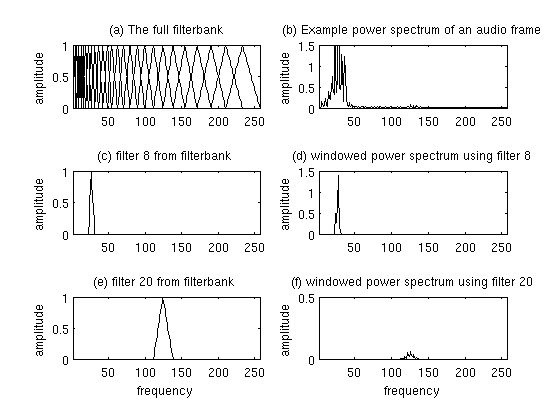
\includegraphics[width=\textwidth]{mel_filterbank_example}
	\caption{Filtering with Mel Filterbanks \cite{practical_cryptography}}
	\label{filterbank}
\end{figure}

\subsection{Log and DCT}
The log of the energies in each filterbank is taken, and a Discrete Cosine Transformation (DCT) is applied to extract 13 new coefficients of this new spectrum. The DCT has several benefits over another transformation like the Fourier transform in that it does not interpret components as infinite waves, and so is better suited where signals are more likely to be interrupted, as the framing process does. Furthermore only real numbers are output which is more readily dealt with by learners such as CNN’s. 
\newline
Generally the largest 13 coefficients are taken that represent the most important information.
https://dsp.stackexchange.com/questions/31/how-do-i-interpret-the-dct-step-in-the-mfcc-extraction-process 
probably need better source…

\subsection{Output}
Hence MFCC’s function as a feature selection technique that reduces the 400 samples each with 256 values ( 8 bits) of amplitude representation to this lower feature space specifically designed to emulate how humans hear, which are themselves well placed to interpret speech signals. However, Figure \ref{mfccs_speech_orno} indicates that the relation between MFCC's and speech presence is not immediately obvious. MFCC2 appears to have the most distinctive correlation with the coefficients doubling in size from $\sim$30 to $\sim$60 in the absence of speech, but other features have similar values, and there is significant intraclass variation.

\begin{figure}[h]
	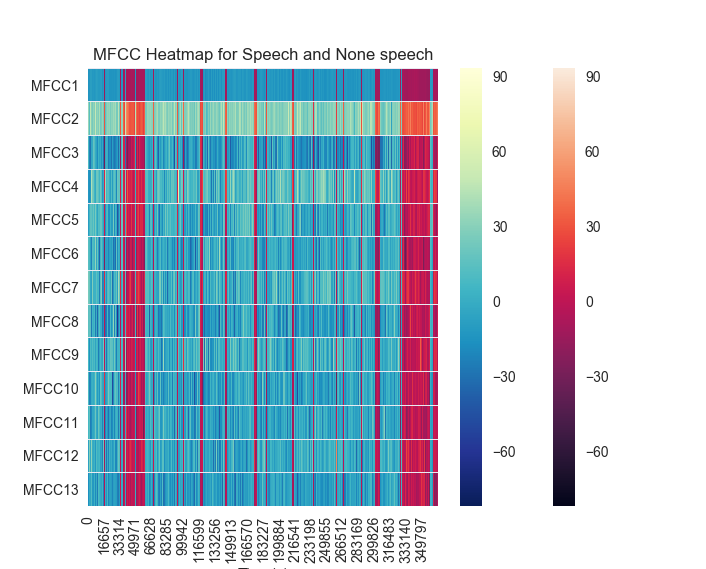
\includegraphics[width=\textwidth]{mfcc_heatmap_speech_or_nospeech}
	\caption{The MFCCs extracted from a Game of Thrones episode. Bluish shades indicate subtitles are absent, pinkish shades indicate they are present. Feature window index is used as a proxy for time.}
	\label{mfccs_speech_orno}
\end{figure}

\section{Subtitles}
The MFCC’s provide the descriptive variables upon which to make predictions, and the objective variable is defined to be the presence of subtitles. This setup was chosen to enable the model to provide based solely on the srt file: since this subtitle synchroniser is aimed principally at cinemagoers, it is assumed that the original audio/video is unavailable, but it is assumed that an srt file is accessible. These are readily available on the internet for most films and are small (essentially text) files and so networking and device requirements would be minimal: they contain a series of entries made up of a start time, stop time, and a string to be presented on the screen at these times. In order to generate the subtitle array:
\begin{itemize}
	\item Times are converted into seconds from start.
	\item The time at which the last subtitle disappears from the screen is used to determine the length in seconds that subtitles are present. Subtitles need only be synchronised when there are actually subtitles present.
	\item The number of frames required is determined by dividing the length in seconds by the frame step (10ms) (the frame length is 25ms, but these are overlapping).
	\item An array of zeros pb\_array is generated with columns for an index, start time and binary subtitle value to indicate presence of subtitles. It is of equal length to the number of frames required.
	\item The 2 arrays, pb\_array and subs\_array, are parsed concurrently, with the frame times of pb\_array checked to see if they lie within a times entry, and the value changed to 1 from 0 if true.
\end{itemize}

\subsection{Pseudocode}
\begin{algorithm}
	\caption{pb\_array\_fill}\label{euclid}
	\begin{algorithmic}[1]
		\Procedure{MyProcedure}{}
		\State $i \gets 0$
		\State $j \gets 0$
		\State $m \gets pb\_array\_length$
		\State $n \gets subs\_array\_length$
		\While {True}
		%\Procedure{Check arrays not exceeded}
		\If {$i > m$ }  
			\BREAK
			\EndIf
		\If {$j > n$ }  
			\BREAK
			\EndIf
		\If {\textit{pb\_array[i] start time} $\geq$ \textit{subs[j] start time}} 
			\If  {\textit{pb\_array[i] end time} $<$ \textit{subs[j] end time}}
				%\COMMENT {Within subs entry}
				\State $pb\_array[i] \gets 1$
				\State $i \gets i+1$
				\EndIf
			%\ELSEIF {$pb\_array[i] end time} $>$ \textit{subs[j] end time}}
			\Else
				\State $j \gets j+1$
			\EndIf
		\EndIf
		\EndProcedure
	\end{algorithmic}
\end{algorithm}

This method was evaluated with 5 trial runs on 59:18 minutes of audio, equating to 355,830 MFCC samples and took on average 12.03 seconds. This is a little longer than would be desired in practice but is not excessively long. This method is efficient in that it parses over the arrays only once.

This outputs a vector with length equal to number of MFCC frames, filled with binary values indicating presence of subtitles. This provides the objective feature to predict.

%----------------------------------------------------------------------------------------

